%\usepackage{amsmath}
%\usepackage{hyperref}
%\usepackage{amsthm}
%\usepackage{graphicx}
\documentclass[journal, a4paper]{IEEEtran}
\usepackage[italian]{babel}
\usepackage{booktabs}
\usepackage{siunitx}%Questo serve a caricare il pacchetto delle unità di misura del sistema internazionale%
\usepackage[utf8]{inputenc}
\usepackage{graphicx} 
\usepackage{url}
\usepackage{amsmath}
\usepackage{amssymb}
\usepackage[lofdepth,lotdepth]{subfig}
\usepackage{textcomp}

\usepackage{keyval}
\usepackage{xcolor}
\usepackage{caption}
\usepackage{tikz}
\usepackage{circuitikz}
\usepackage{authblk}
%\usepackage{subcaption}
%\usepackage{hyperref}

\begin{document}


% Define document title and author
	\title{Tecnologie Digitali - Logbook Week 11}
	\author[1]{Salvatore Bottaro}
		\author[2]{Lorenzo M. Perrone}
		\affil[1]{\texttt{salvo.bottaro@hotmail.it}}
		\affil[2]{\texttt{lorenzo.perrone.lmp@gmail.com}}
	\markboth{Tecnologie Digitali - Di Lieto}{}
	\maketitle
	
\begin{abstract}
	Logbook di laboratorio di Tecnologie Digitali, a.a. 2015/2016. Week 11.
\end{abstract}

\section{Divisore per 3}
Combinando opportunamente uno o due \textit{flip-flop} è possibile realizzare dei divisori di frequenza non necessariamente multipli di 2. Un esempio è il cd. \textbf{divisore per 3} che si ottiene collegando due \textit{flip-flop} di tipo \textsc{D} fra loro con un circuito \textsc{NAND}, come mostrato in Figura (\ref{fig:es9}).\\

\begin{figure}
\centering
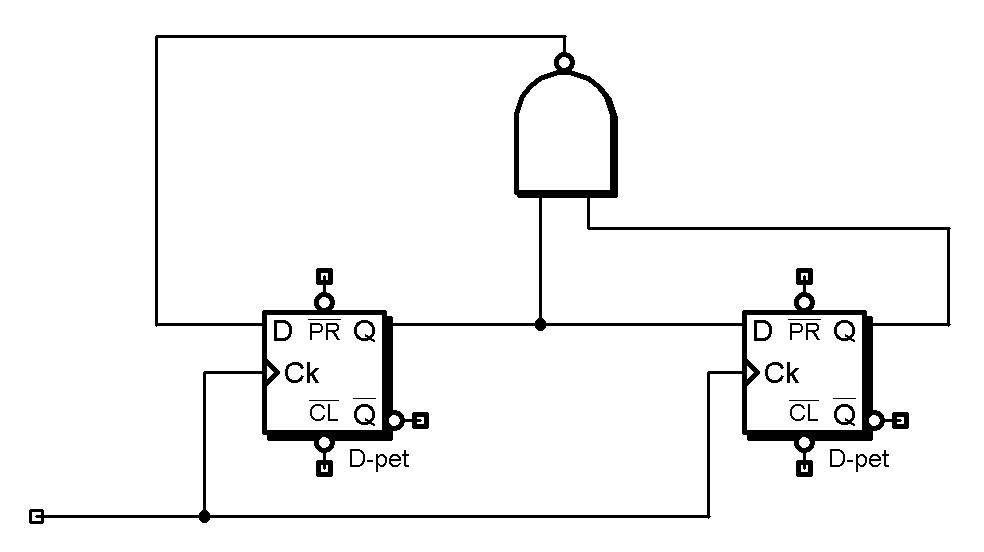
\includegraphics[width=0.8\linewidth]{./es9_mono}
\caption{Circuito divisore per 3}
\label{fig:es9}
\end{figure}

Siano contrassegnati con il numero "1" tutti gli i/o del primo \textit{flip-flop}, con il numero "2" quelli del secondo. In particolare, è facile verificare a vista che $D2 = Q1$ e che $D1 = \lnot(Q1 \cdot Q2)$. Per ogni fronte d'onda di risalita del \textit{clock}, tale per cui si verifica un aggiornamento delle assegnazioni delle uscite e degli ingressi, possiamo scrivere una sequenza di stati come segue:\\

\begin{table}[h]
\centering
\begin{tabular}{c|c||c|c}
\hline \textbf{D1} & \textbf{Q1} & \textbf{D2} & \textbf{Q2} \\ 
\hline 0 & 1 & 1 & 1 \\ 
 1 & 0 & 0 & 1 \\
 1 & 1 & 1 & 0 \\ 
 0 & 1 & 1 & 1 \\ 
 1 & 0 & 0 & 1 \\
 1 & 1 & 1 & 0 \\
 
\hline
 
\end{tabular} 
\end{table}
~\\

Si nota che le assegnazioni alla terza riga sono le stesse della riga sei, per cui si ha un ciclo della durata di 3 fronti di risalita del \textit{clock}, il che è evidentemente in accordo con la denominazione di \textit{divisore per 3} di tale circuito. Se guardiamo i valori assunti, ad esempio, dall'uscita $Q2$ vediamo che si tratta di una sequenza di acceso/spento asimmetrica, in cui $1/3$ del periodo complessivo è passato nello stato spento, i restanti $2/3$ in quello di acceso (discorso analogo vale per l'uscita $Q1$).\\
Proviamo ora a montare sulla breadboard il circuito e verificare con il tester digitale il suo effettivo funzionamento. La frequenza di clock viene data azionando manualmente l'interruttore della \textsc{cb49} tramite il VI \textsc{Digital\_out4}. Per ogni accensione \textbf{e} spegnimento dell'interruttore apposito, l'uscita dalla $Q2$ è come segue:

\begin{equation}
1\,1\,1\,1\,0\,0\,1\,1\,1\,1\,0\,0\,1\,1\,1\,1\,0\,0
\end{equation}

In altre parole, si verifica praticamente che soltanto il fronte d'onda di risalita del clock aggiorna le uscite, mentre invece quello di discesa le lascia invariate (si veda la \textsc{truth table} del flip-flop MC14013B riportata nel datasheet \cite{M06}).\\
Connettiamo ora l'uscita $Q2$ al contatore della scheda DAQ posto alla \textsc{CB3}, la frequenza di clock ora è data dal generatore di funzioni, e usiamo il VI \textsc{Contatore\_freq} per misurare la frequenza in uscita dal circuito. La $f_{CLK} = 25.78$kHz, ci aspettiamo quindi che $f_{Q2}$ sia circa un terzo della prima. L'istogramma restituito dal VI è in Figura () e le frequenze prevalenti su 100 campionamenti sono circa $f_{Q2} \simeq $8.6kHz in accordo con quanto previsto. E' certamente corretto affermare che dal punto di vista della frequenza il circuito sia un divisore per tre, ma è altrettanto evidente che l'uscita è fortemente asimmetrica (più avanti si approfondirà questo aspetto).\\

Può essere interesante verificare questi stessi risultati usando gli ingressi analogici della \textsc{DAQ}, visualizzando l'ingresso e l'uscita (in due tempi, separatamente) con il VI \textsc{acquis\_base\_2015}. Si è collegato prima, quindi, l'ingresso del generatore di funzioni alla \textsc{cb68}, e in secondo luogo l'uscita $Q2$. La frequenza del segnale di clock è $f_{CLK} \simeq 7$kHz, quella di campionamento è di 200kSample/s, la durata di campionamento (la stessa per entrambe le rilevazioni) è stata di $d = 0.001s$, con un fondoscala di 10V. In Figura (\ref{fig:es12_prova}) è riportato il multiplot con entrambi i segnali.\\
E' interessante evidenziare come i due livelli \textit{acceso} non siano proprio uguali, ma ci sia uno scarto di circa 250mV, probabilmente dovuto ai differenti range dei segnali di output (in tensione) fra i \textit{flip-flop} e il \textsc{NAND}.\\

\begin{figure}
\centering
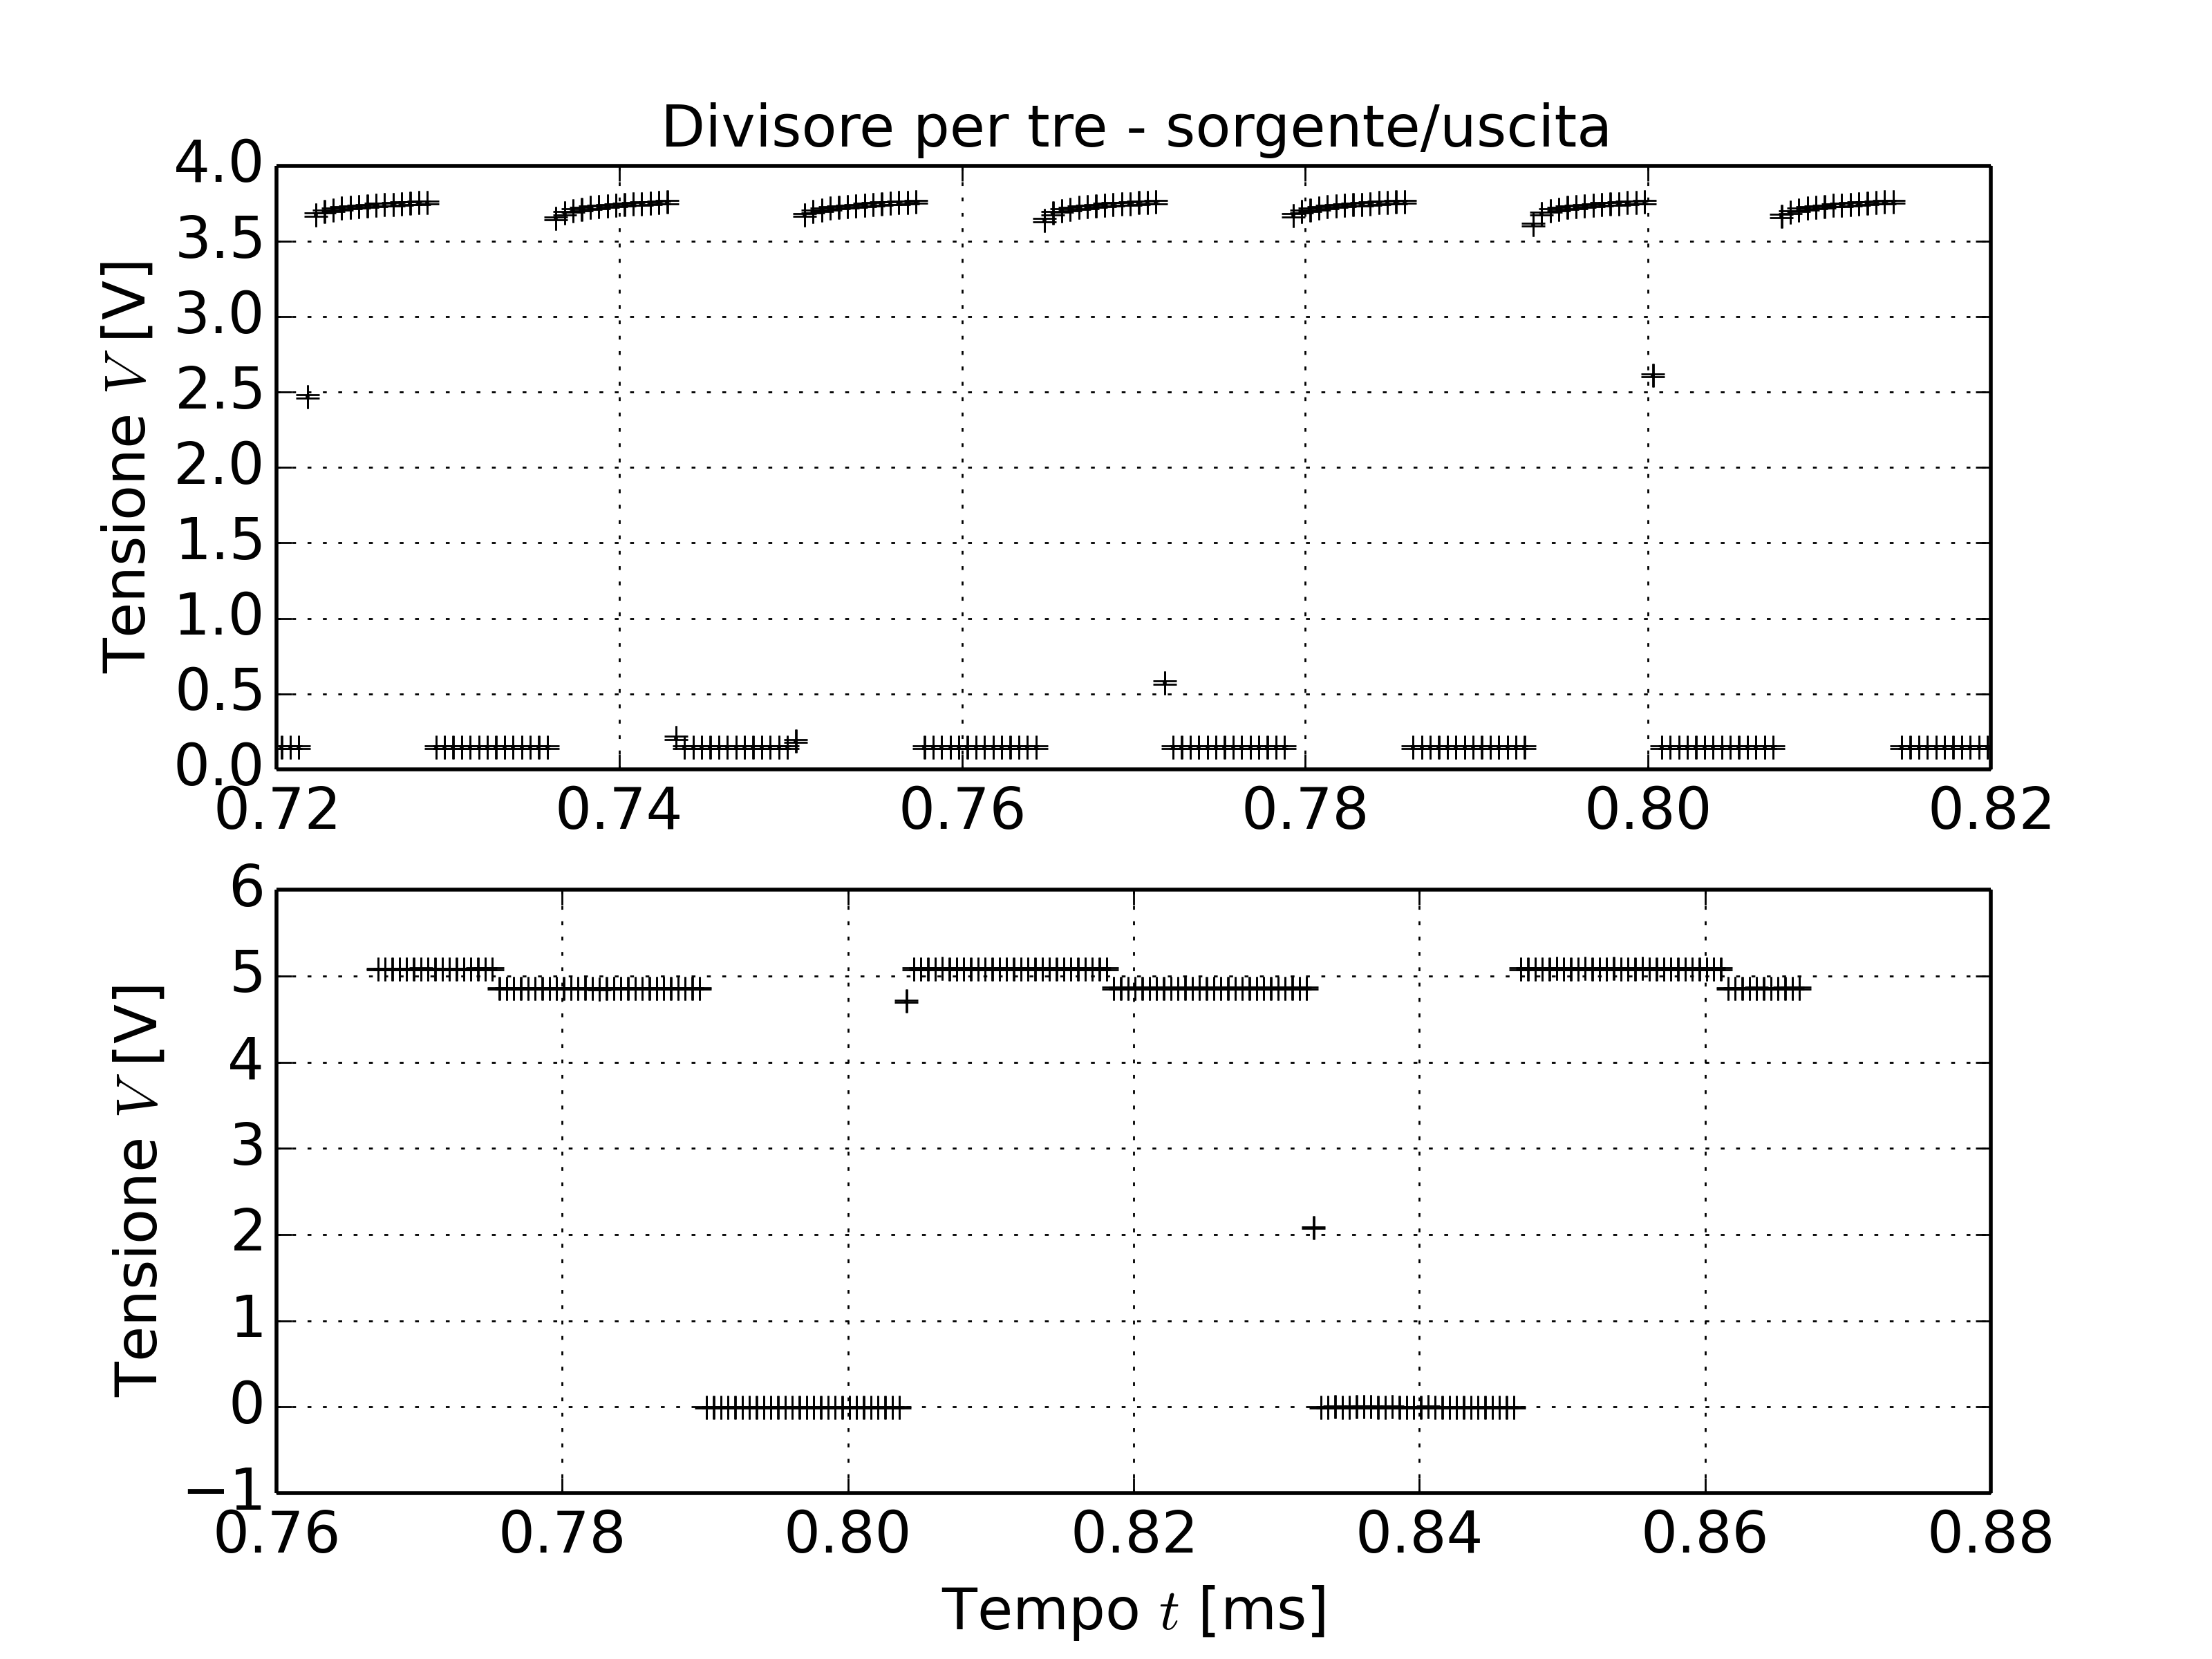
\includegraphics[width=0.8\linewidth]{./es12_prova}
\caption{Divisore per tre - acquisizione analogica segnale e uscita}
\label{fig:es12_prova}
\end{figure}

Andiamo ora ad esaminare con maggiore attenzione l'asimmetria dell'uscita del nostro circuito introducendo la nozione di \textit{duty cycle} ($\eta$). Se chiamiamo $T1$ e $T2$ rispettivamente il tempo in cui il segnale si trova acceso (\textbf{TRUE}) o spento (\textbf{FALSE}), il \textit{duty cycle} è definito come:

\begin{equation}
\eta = \frac{T1}{T1 + T2}
\end{equation}

Nel caso di segnali simmetrici, $\eta$ è ovviamente 0.5. Tramite il VI \textsc{Contatore\_pulsew} si può verificare che il \textit{duty-cycle} del segnale prodotto dal generatore di funzioni sia circa 1/2. I risultati ottenuti per il \textit{falling time} e per il \textit{rising time} sono, rispettivamente, di $t_F = 7.123(5)E-5 s$ e $t_R = 7.130(5)E-5 s$, che risultano in $\eta = 0.5002$.\\
Se proviamo a misurare le stesse grandezze per il segnale prodotto dal divisore per tre, i risultati sono: 

\begin{table}[h]
\centering
\begin{tabular}{c|c}
\hline \textbf{falling time} & \textbf{rising time} \\ 
 1.3E-4 s & 2.6E-4 s \\ 
\hline 
\end{tabular}   
\end{table}
~\\
In linea con quanto ci aspettiamo. Bisogna notare, tuttavia, che per acquisire questi risultati si sono avute delle difficoltà dovute alla presenza di segnali ad alta frequenza nelle uscite che hanno \textit{sporcato} l'output del circuito e hanno spesso prodotto degli errori nel funzionamento del VI. 

\subsection{Hw. 4}
Vediamo come si comporterebbe il divisore per 3 se al posto di un circuito \textsc{NAND} mettessimo un \textsc{NOR}. Possiamo ipotizzare che il comportamento non sia troppo dissimile, dal momento che sia il \textsc{NAND} che il \textsc{NOR} prevedono un'uscita \textit{simmetrica} fra di loro:

\begin{table}[h]
\centering
\begin{tabular}{c|c||c|c}
\hline \textbf{A} & \textbf{B} & \textbf{NAND(A,B)} & \textbf{NOR(A,B)} \\ 
\hline 1 & 1 & 0 & 0 \\ 
 1 & 0 & 1 & 0 \\ 
 0 & 1 & 1 & 0 \\ 
 0 & 0 & 1 & 1 \\ 
\hline
 
\end{tabular} 
\end{table}
~\\
Verifichiamo se l'intuizione è giusta (o meno) preparando una tavola della verità come in precedenza (dove questa volta D1 = NOR(Q1,Q2) e D2=Q1):

\begin{table}[h]
\centering
\begin{tabular}{c|c||c|c}
\hline \textbf{D1} & \textbf{Q1} & \textbf{D2} & \textbf{Q2} \\ 
\hline 0 & 1 & 1 & 1 \\ 
 0 & 0 & 0 & 1 \\
 1 & 0 & 0 & 0 \\ 
 0 & 1 & 1 & 0 \\ 
 0 & 0 & 0 & 1 \\
 1 & 0 & 0 & 0 \\
 0 & 1 & 0 & 0\\
 
\hline
 \end{tabular} 
\end{table}
~\\
Come si vede, il circuito funziona sempre da divisore per tre, dove però per 2/3 del periodo lo stato è \textbf{FALSE} e per 1/3 è \textbf{TRUE} (i ruoli sono invertiti). Il \textit{duty cycle} per questa configurazione sarebbe allora $\eta = 0.66$ invece che $\eta = 0.33$.

\section{Simmetrizzatore}
A questo punto vogliamo  provare ad integrare il circuito precedente in modo da simmetrizzare il segnale di uscita e ottenere dunque un \textbf{divisore per 3 simmetrico}. Per fare questo, c'è bisogno di aggiungere ai due flip flop un ulteriore flip flop con un circuito \textsc{NOR}. Questi ultimi due da soli costituiscono il simmetrizzatore, e sono rappresentati in Figura (\ref{fig:es15_simmet}).\\

\begin{figure}
\centering
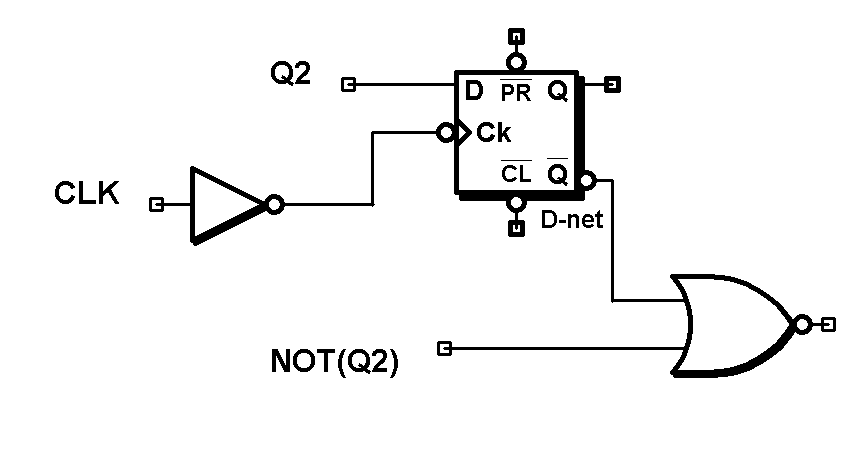
\includegraphics[width=0.8\linewidth]{./es15_simmet}
\caption{Circuito simmetrizzatore}
\label{fig:es15_simmet}
\end{figure}


Un aspetto importante è che il segnale di clock questa volta viene dato \underline{negato} al flip flop. Per capire il motivo di questa scelta trascriviamo la tavola di verità del circuito simmetrizzatore, utilizzando come ingresso l'uscita $Q2$ del divisore per tre, e il segnale di clock opportuno:


\begin{table}[h]
\centering
\begin{tabular}{c|c|c|c|c|c|c|c}
\hline \textbf{CLK} & \textbf{Q2=D} & \textbf{$\lnot CLK$} & \textbf{Q} & \textbf{Q(CLK)}& \textbf{$\lnot Q$} & \textbf{$\lnot Q2$} & \textbf{NOR($\lnot Q2, \lnot Q1)$} \\ 
\hline
 1 & 1 & 0 & -& 1& -& 0 & -\\ 
 0 & 1 & 1 & 1& 1& 0& 0 & 1\\
 1 & 1 & 0 & 1& 1& 0& 0 & 1\\ 
 0 & 1 & 1 & 1& 1& 0& 0 & 1\\ 
 1 & 0 & 0 & 1& 0& 0& 1 & 0\\
 0 & 0 & 1 & 0& 0& 1& 1 & 0\\
 1 & 1 & 0 & 0& 1& 1& 0 & 0\\
 0 & 1 & 1 & 1& 1& 0& 0 & 1\\
 \hline
\end{tabular} 
\end{table}
~\\

Come si nota, se dessimo il segnale non negato di clock, in uscita \textbf{Q(CLK)} otterremmo lo stesso ingresso \textbf{Q2}. L'effetto del $\lnot CLK$  è quello di shiftare verso il basso l'uscita rispetto all'ingresso. Come risultato, l'output del circuito simmetrizzatore è una sequenza simmetrica 000111000 con frequenza tripla rispetto a quella di clock (ricordiamo che l'aggiornamento del'uscita è ad ogni fronte d'onda di salita, per cui in quelli di discesa essa non varia).\\


\begin{figure}
\centering
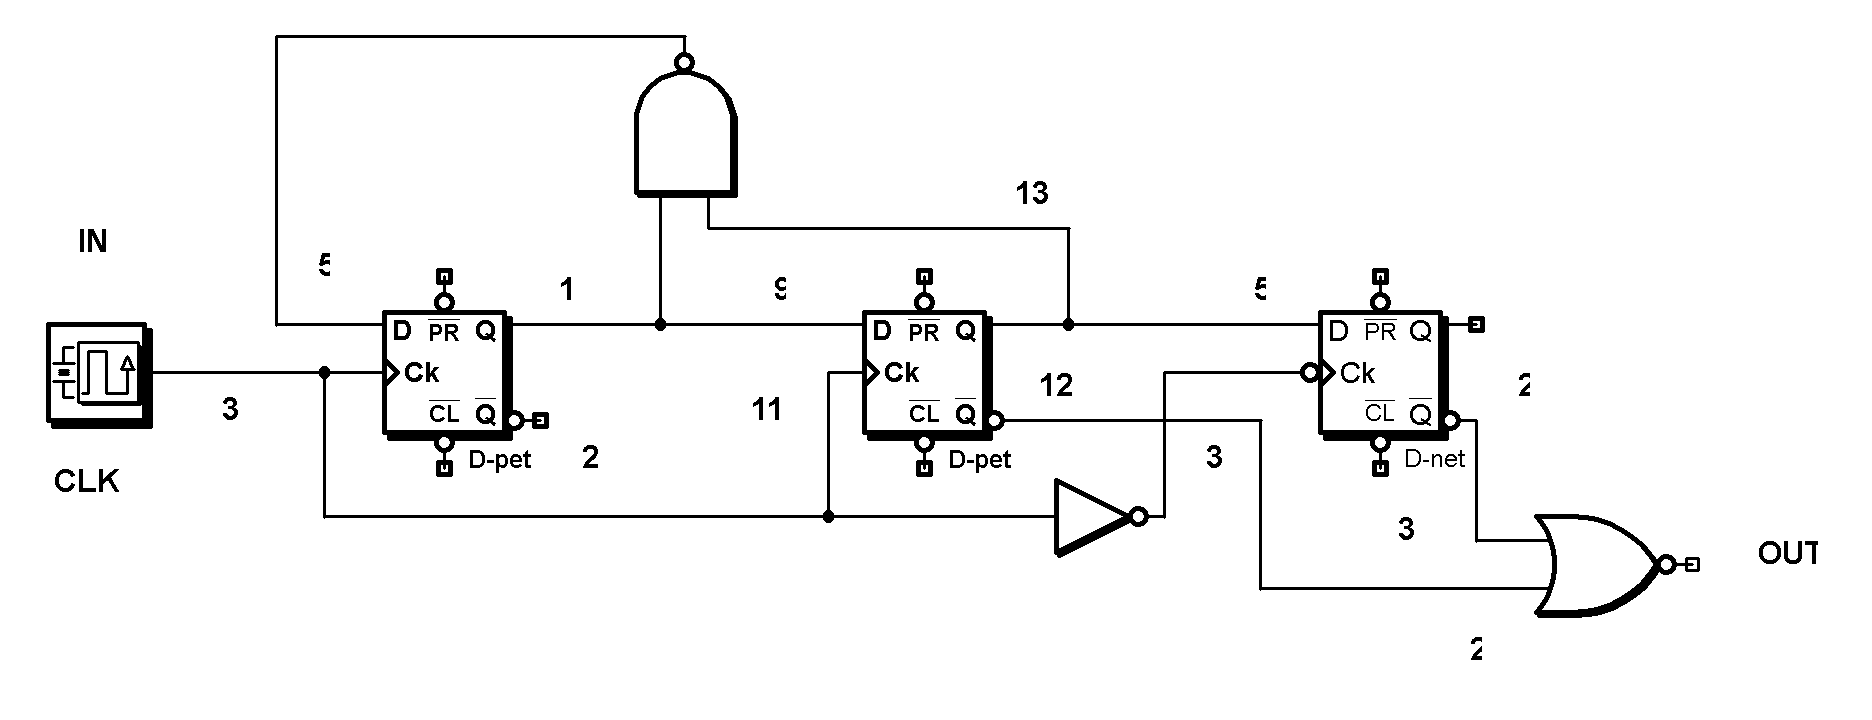
\includegraphics[width=0.9\linewidth]{./es16_circ_simm}
\caption{Circuito divisore per 3 + simmetrizzatore.}
\label{fig:es16_circ_simm}
\end{figure}


Verifichiamo adesso, montando il simmetrizzatore in sequenza al divisore per tre, il corretto funzionamento del circuito (Figura (\ref{fig:es16_circ_simm})). La fase di montaggio è stata particolarmente ostica, a causa dell'elevato numero di connessioni fra i diversi pin dei componenti. In particolare, nella fase di debug, abbiamo incontrato difficoltà nel capire un malfunzionamento del circuito, che alla fine (inspiegabilmente) si è risolto da solo: durante i primi tentativi sembrava che l'alimentazione dei componenti (dalla \textsc{cb14}) fosse data in alternata e non in continua. Ad ogni modo, dopo aver sistemato il circuito, il risultato del campionamento dell'ingresso e dell'uscita è mostrato nelle Figure (\ref{fig:es16_senzaline}, \ref{fig:es16_conline}). La frequenza di acquisizione è stata di 100kS/s, per una durata complessiva di 0.003s.

\begin{figure}
\centering
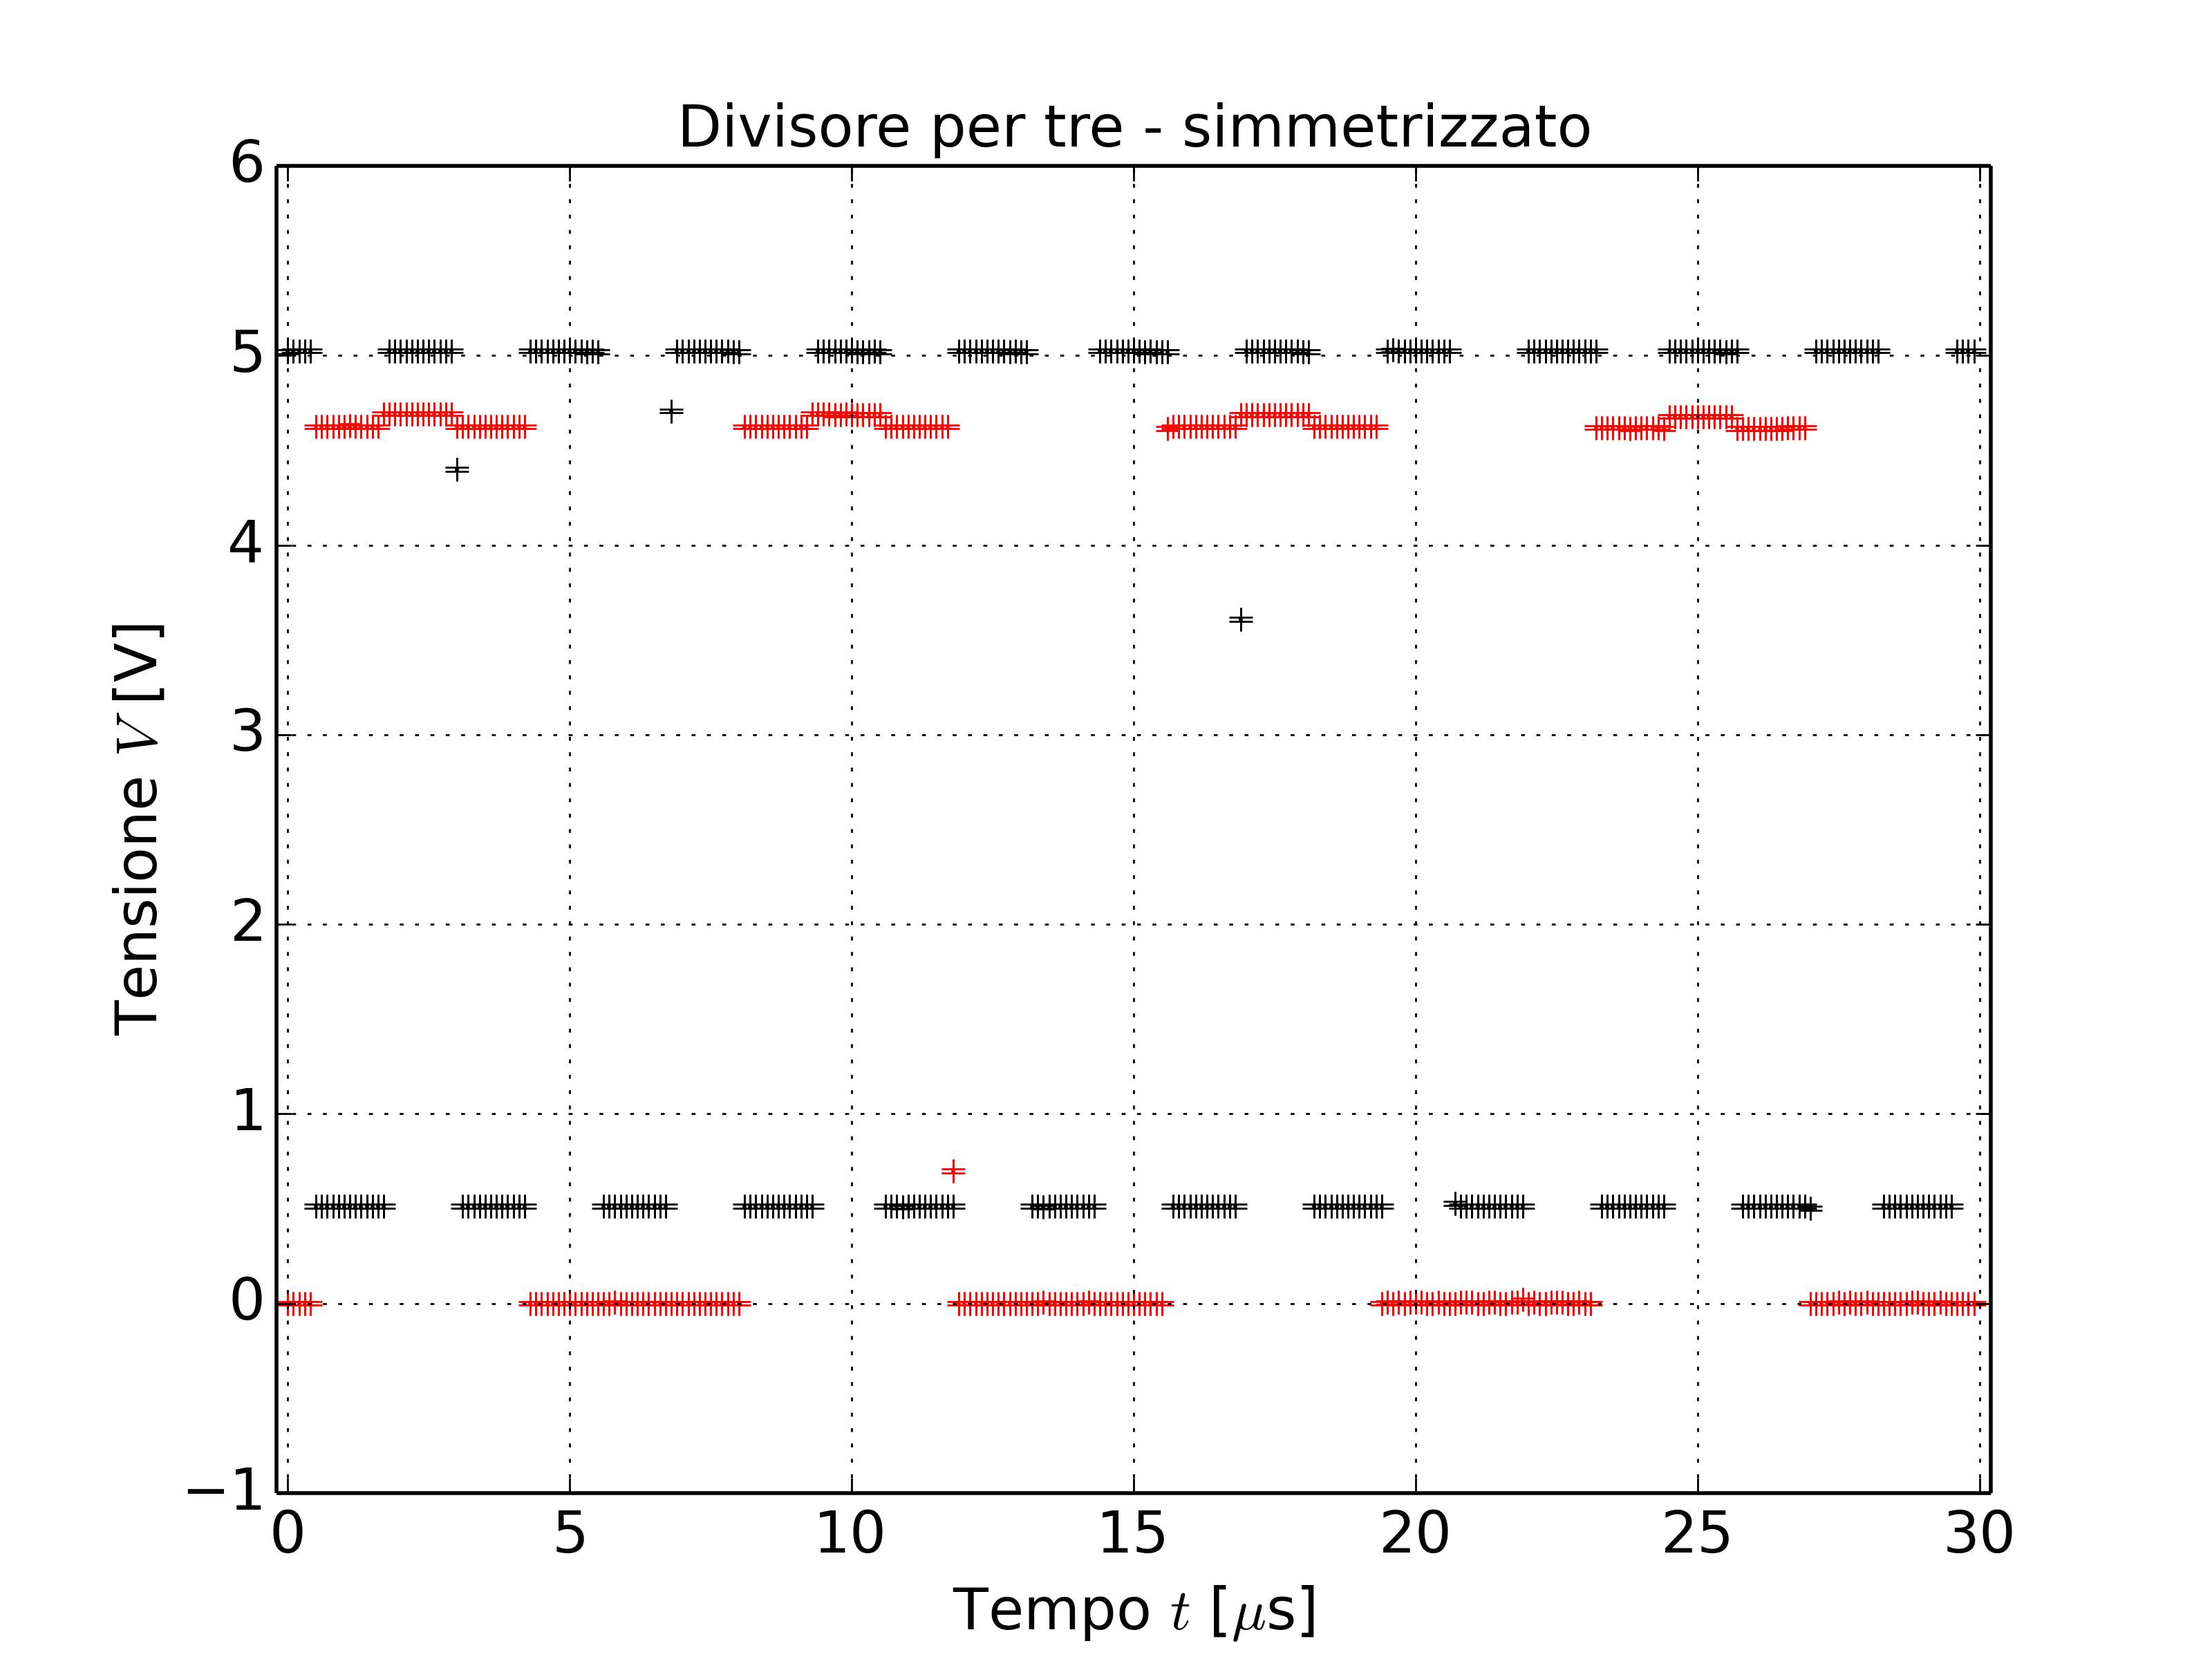
\includegraphics[width=0.9\linewidth]{./es16_senzaline}
\caption{Divisore per 3 simmetrizzato - senza linea}
\label{fig:es16_senzaline}
\end{figure}


\begin{figure}
\centering
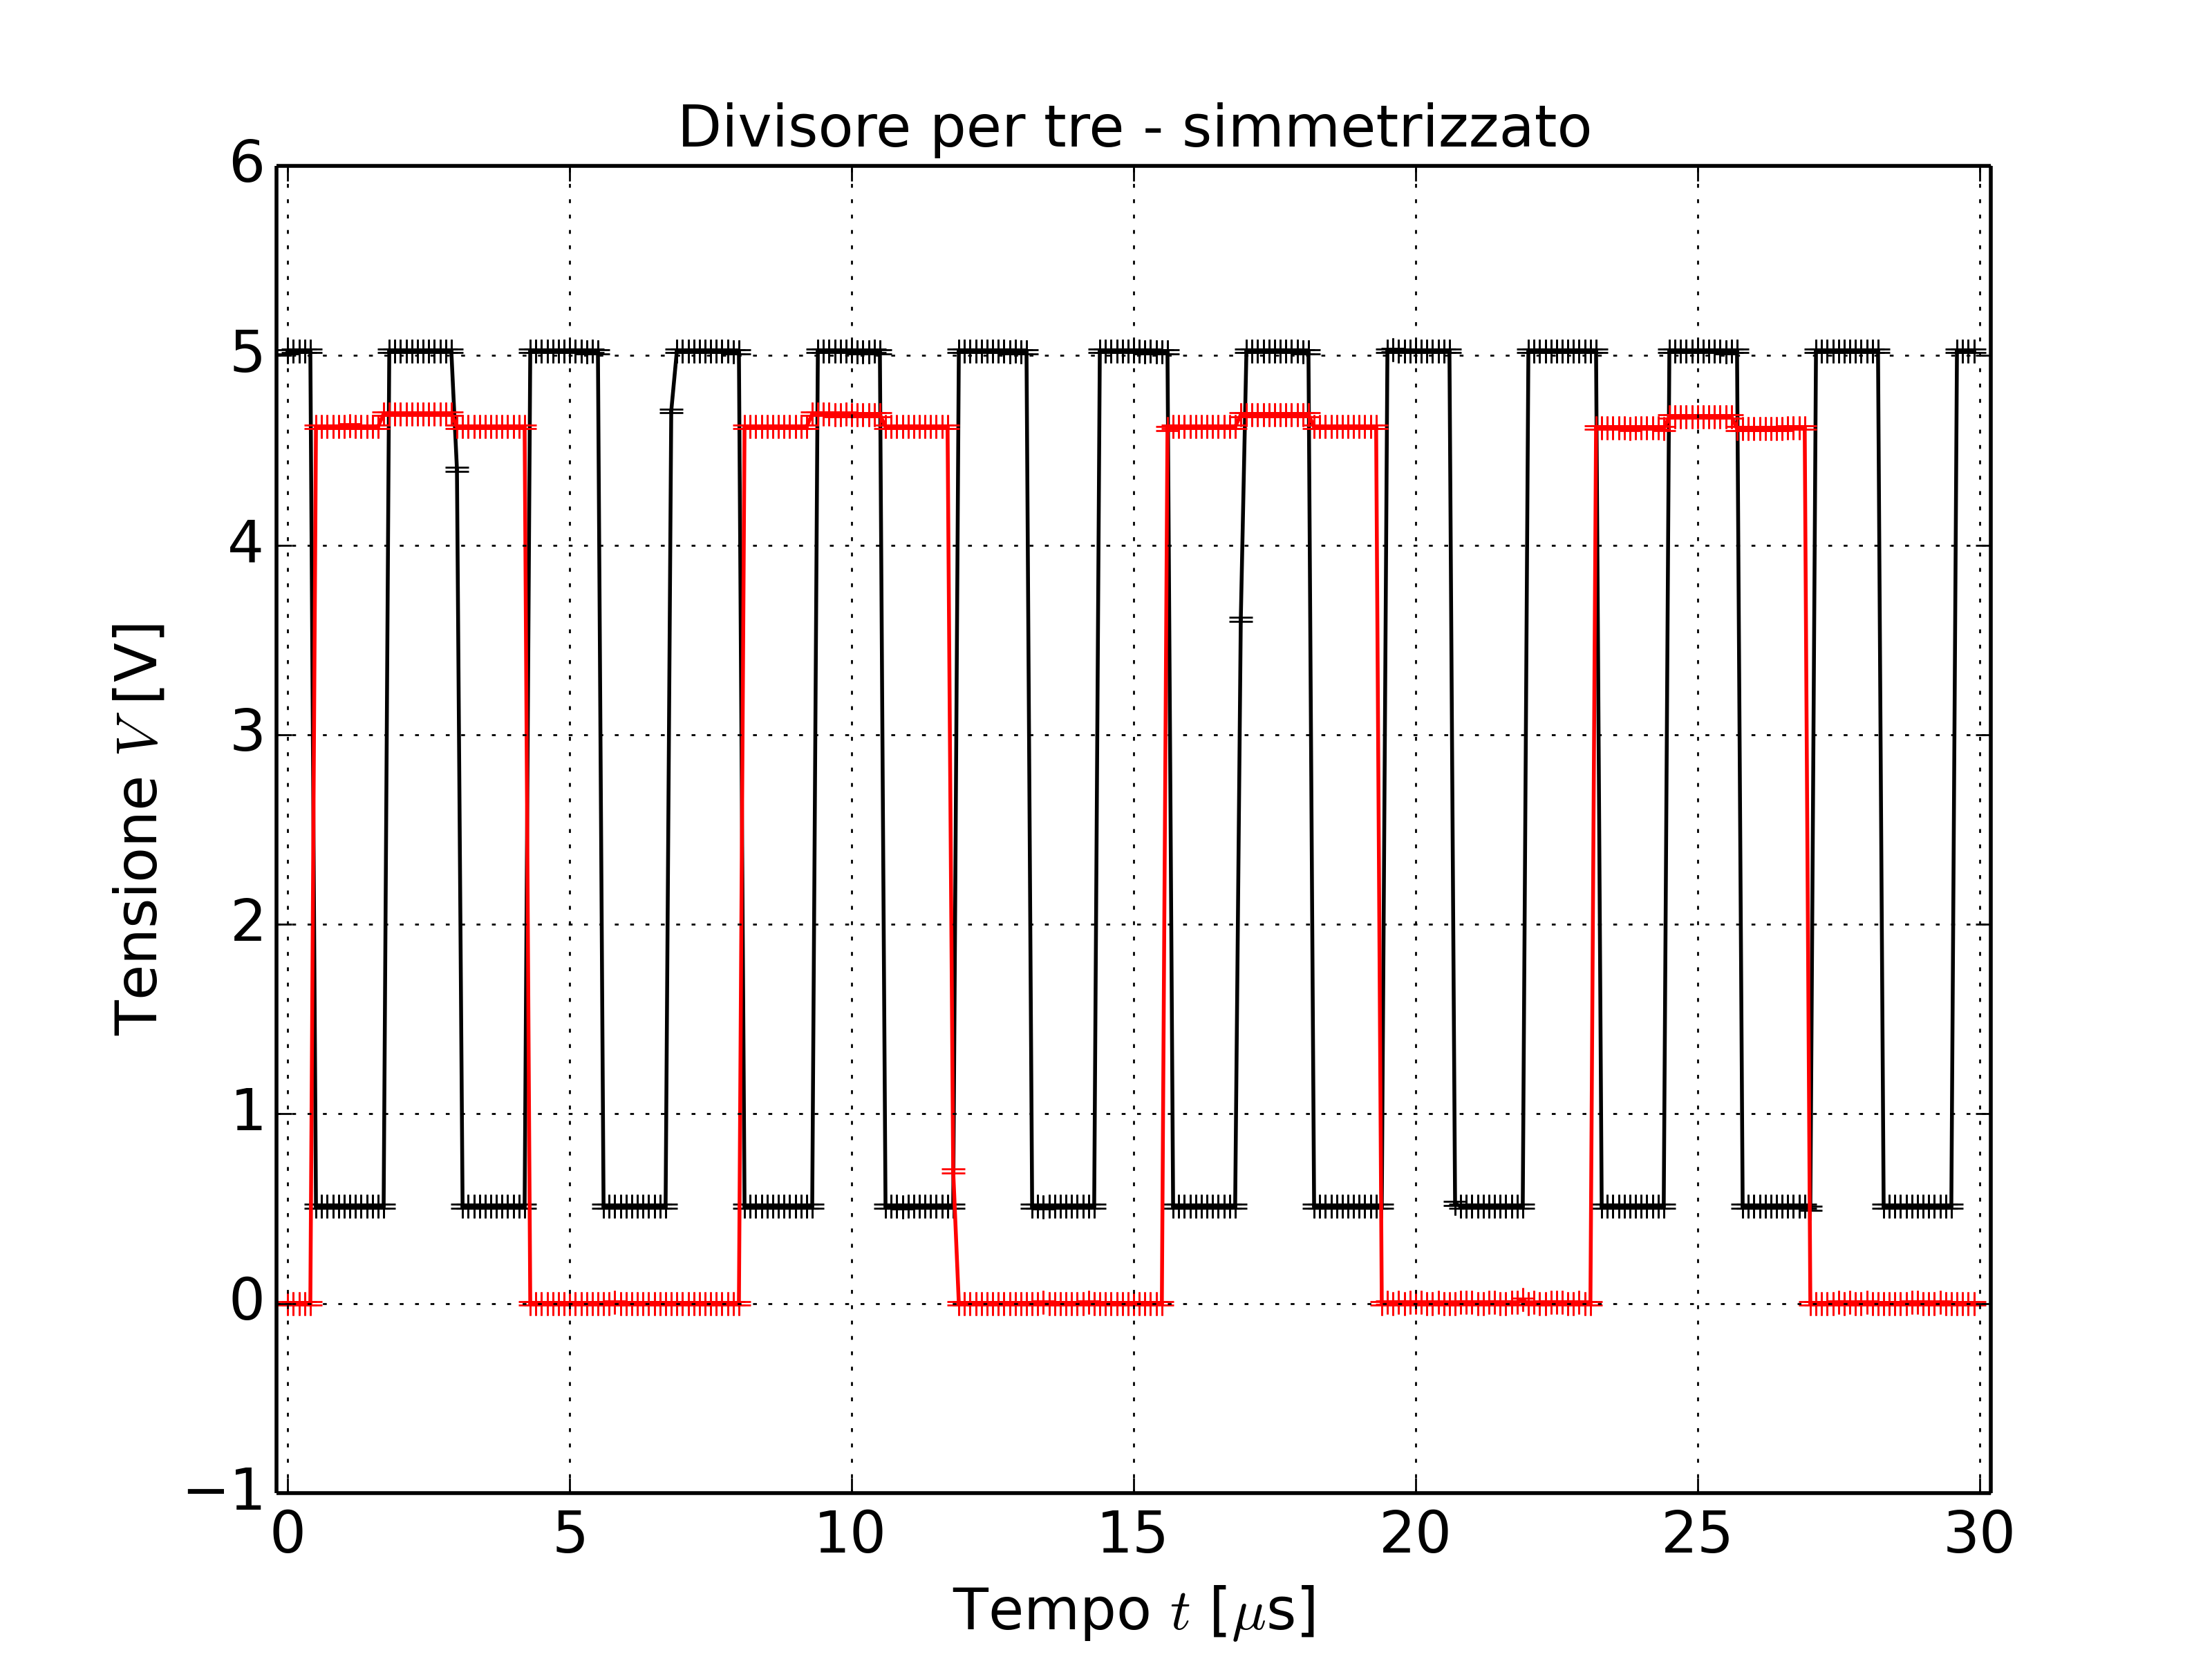
\includegraphics[width=0.9\linewidth]{./es16_conline}
\caption{Divisore per tre simmetrizzato - con linea}
\label{fig:es16_conline}
\end{figure}


\subsection{Hw. 5}
Un modo per costruire un simmetrizzatore con porta \textsc{NAND} per un divisore per tre, consiste nell'impiegare la variante \textsc{nor} di tale divisore, e sostituire il \textsc{nor} con un \textsc{nand} nel simmetrizzatore. Si può vedere lo schema in Figura (\ref{fig:hw5}). Invece, la tavola di verità è la seguente:

\begin{table}[h]
\centering
\begin{tabular}{c|c|c|c|c|c|c|c}
\hline \textbf{CLK} & \textbf{Q2=D} & \textbf{$\lnot CLK$} & \textbf{Q} & \textbf{Q(CLK)}& \textbf{$\lnot Q$} & \textbf{$\lnot Q2$} & \textbf{NAND($\lnot Q2, \lnot Q1)$} \\ 
\hline
 1 & 0 & 0 & -& 1& -& 1 & -\\ 
 0 & 0 & 1 & 0& 1& 1& 1 & 0\\
 1 & 0 & 0 & 0& 1& 1& 1 & 0\\ 
 0 & 0 & 1 & 0& 1& 1& 1 & 0\\ 
 1 & 1 & 0 & 0& 0& 1& 0 & 1\\
 0 & 1 & 1 & 1& 0& 0& 0 & 1\\
 1 & 0 & 0 & 1& 1& 0& 1 & 1\\
 0 & 0 & 1 & 0& 1& 1& 1 & 0\\
 \hline
\end{tabular} 
\end{table}
~\\


\begin{figure}
\centering
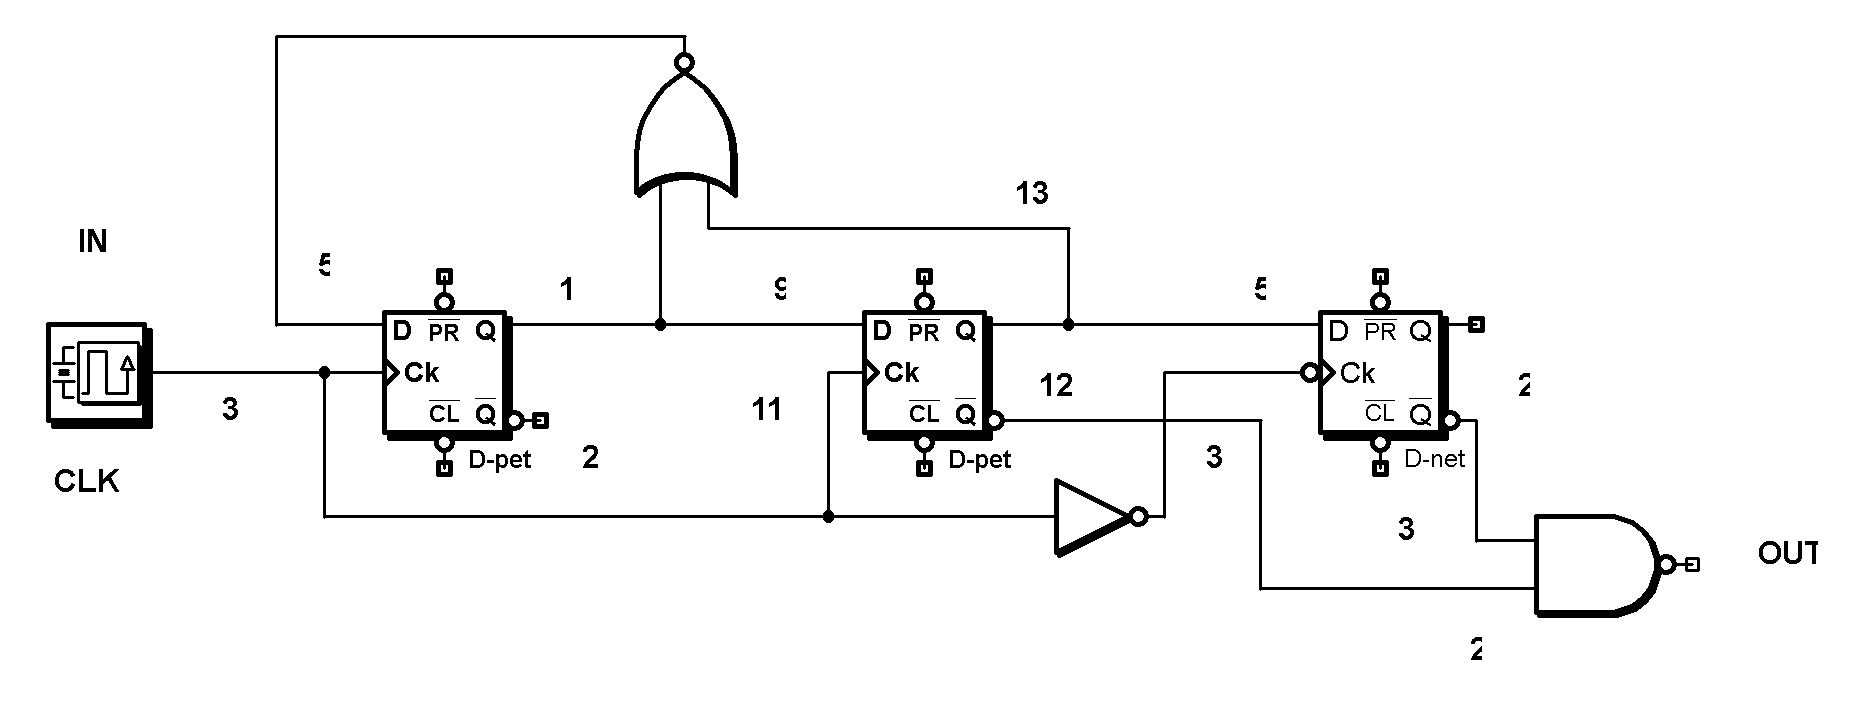
\includegraphics[width=0.9\linewidth]{./hw5}
\caption{Divisore per tre + simmetrizzatore NAND}
\label{fig:hw5}
\end{figure}


\begin{thebibliography}{5}

	%Each item starts with a \bibitem{reference} command and the details thereafter.
	
	\bibitem{JH6} % Conference paper
	Product data sheet: Dual Type D Flip-Flop \textsc{mc14013b}.
	\url{http://onsemi.com}

	\bibitem{M06} % Conference paper
	Paul Horowitz, Winfield Hill - The Art of Electronics. Cambridge University Press (1989).
	
\end{thebibliography}

\end{document}